\chapter{\IfLanguageName{dutch}{Figuren: Ontwikkeling Van Het Prototype}{Prototype: Development}}%
\label{ch:stappenplan-prototype}

\begin{figure}[H]
	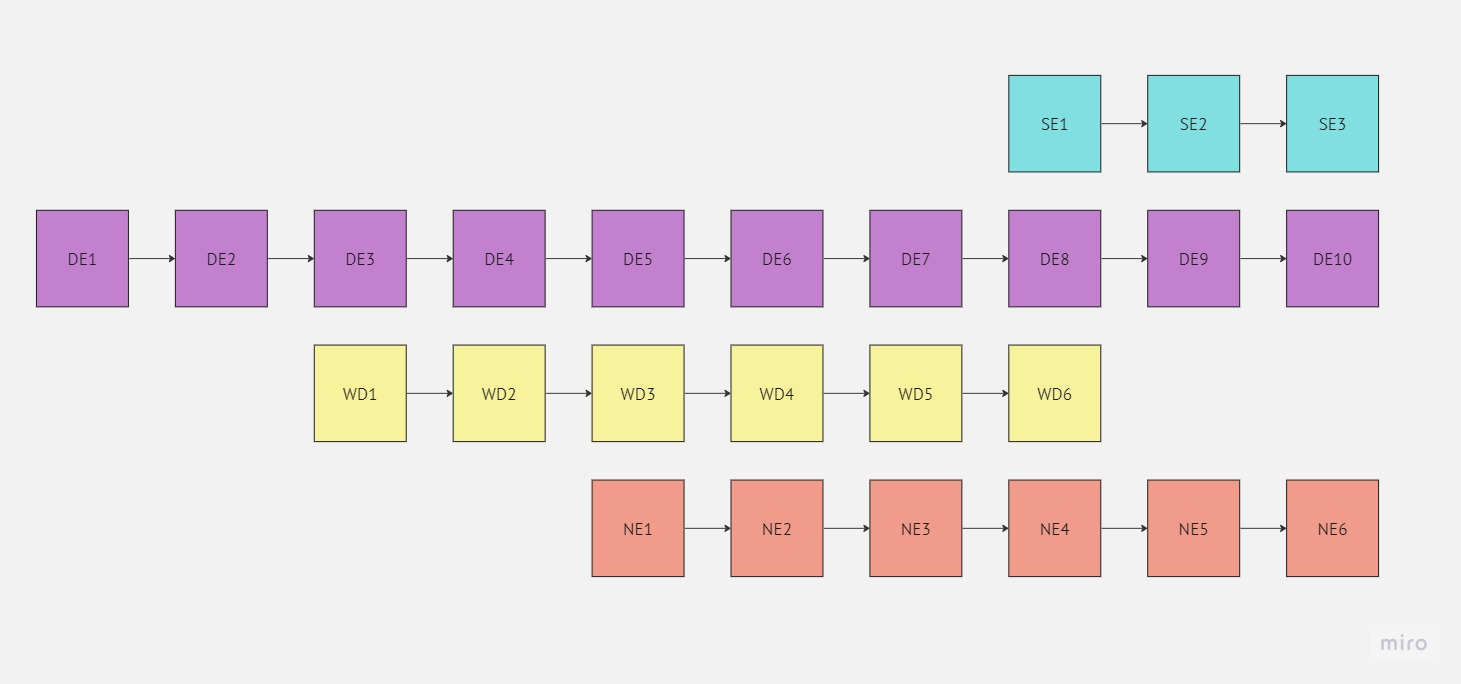
\includegraphics[width=\linewidth]{img/flowchart-development.jpg}
	\caption{Stappenplan voor de ontwikkeling van het component voor lectoren.}
	\label{img:stappenplan-leerkrachten}
\end{figure}

\begin{center}
	\begin{table}
		\begin{tabular}{ | m{2cm} | m{12cm} | } 
			\hline
			WD1 & Flask-skelet aanmaken \\
			WD2 & Formulier voor GPT-3 API-sleutel invoer maken + sessie \\
			WD3 & Formulier voor gepersonaliseerde opties van website aanmaken + sessie \\
			WD4 & Webpagina's aanmaken in HTML \& CSS \\
			WD5 & Invoerformulier maken voor PDF- en tekstupload \\
			WD6 & Invoerformulier maken voor het genereren van een gepersonaliseerde vereenvoudiging van een wetenschappelijk artikel \\
			\hline
		\end{tabular}
		\caption{Taken van de webontwikkelaar bij het uitwerken van het lerarencomponent.}
		\label{table:tasks-web-engineer}
	\end{table}
\end{center}

\begin{center}
	\begin{table}[H]
		\begin{tabular}{ | m{2cm} | m{12cm} | } 
			\hline
			NE1 & Spacy word embeddings laden \&PoS-tagging en lemmatization implementeren \\
			NE2 & Dictionary implementen voor het bijhouden van de PoS-tag per dictionary \\
			NE3 & Jupyter notebook om gepersonaliseerde prompts en aangepaste hyperparameters uit te testen voor de GPT-3 API \\
			NE4 & Jupyter notebook gebruiken om tekstvereenvoudigingsfuncties met GPT-3 API uit te testen. \\
			NE5 & Optioneel: Extra trainingsdata toevoegen aan GPT-3 model. \\
			NE6 & Code voor de voorgestelde pipeline voor ATS implementeren in Python back-end. \\
			\hline
		\end{tabular}
		\caption{Taken van de NLP Engineer bij het uitwerken van het lerarencomponent.}
		\label{table:tasks-nlp-engineer}
	\end{table}
\end{center}


\begin{center}
	\begin{table}[H]
		\begin{tabular}{|m{2cm}|m{12cm}|}
			\hline
			DE1	& Python-notebook om PDFMiner uit te testen bij willekeurige wetenschappelijke artikelen (2000 - nu) \\
			DE2 & Python-notebook opstellen om EasyOCR uit te testen bij willekeurige wetenschappelijke artikelen \\
			DE3 & Jupyter notebook om tekstdata cleaning te realiseren. De restanten van de PDF-extractie moeten weg. \\
			DE4 & Jupyter notebook om look-up methode voor synoniemen te realiseren. \\
			DE5 & Code in back-end implementeren voor PDF-upload via in-memory PDF read. \\
			DE6 & Python-notebook om Pandoc PDF \& Word-document te genereren. \\
			DE7 & Uittesten van YAML-header in Markdown-bestand voor een document op maat. \\
			DE8 & Uittesten van uitschrijven tekstinhoud naar Markdown-bestand \\
			DE9 & Implementatie code van Pandoc in Flask-framework \\
			DE10 & Code in back-end implementeren voor zippen \& doorsturen naar eindgebruiker. \\
			\hline
		\end{tabular}
		\caption{Taken van data engineer bij het uitwerken van het lerarencomponent.}
		\label{table:tasks-data-engineer}
	\end{table}
\end{center}

\begin{center}
	\begin{table}
		\begin{tabular}{|m{2cm}|m{12cm}|}
			\hline
			SE1 & Dockerfile en bijhorende requirementsfile aanmaken \\
			SE2 & Opzet in Docker realiseren \\
			SE3 & Powershell en Bash-script realiseren \\
			\hline
		\end{tabular}
		\caption{Taken van de system engineer bij het uitwerken van het lerarencomponent.}
		\label{table:tasks-system-engineer}
	\end{table}
\end{center}

\begin{figure}[H]
	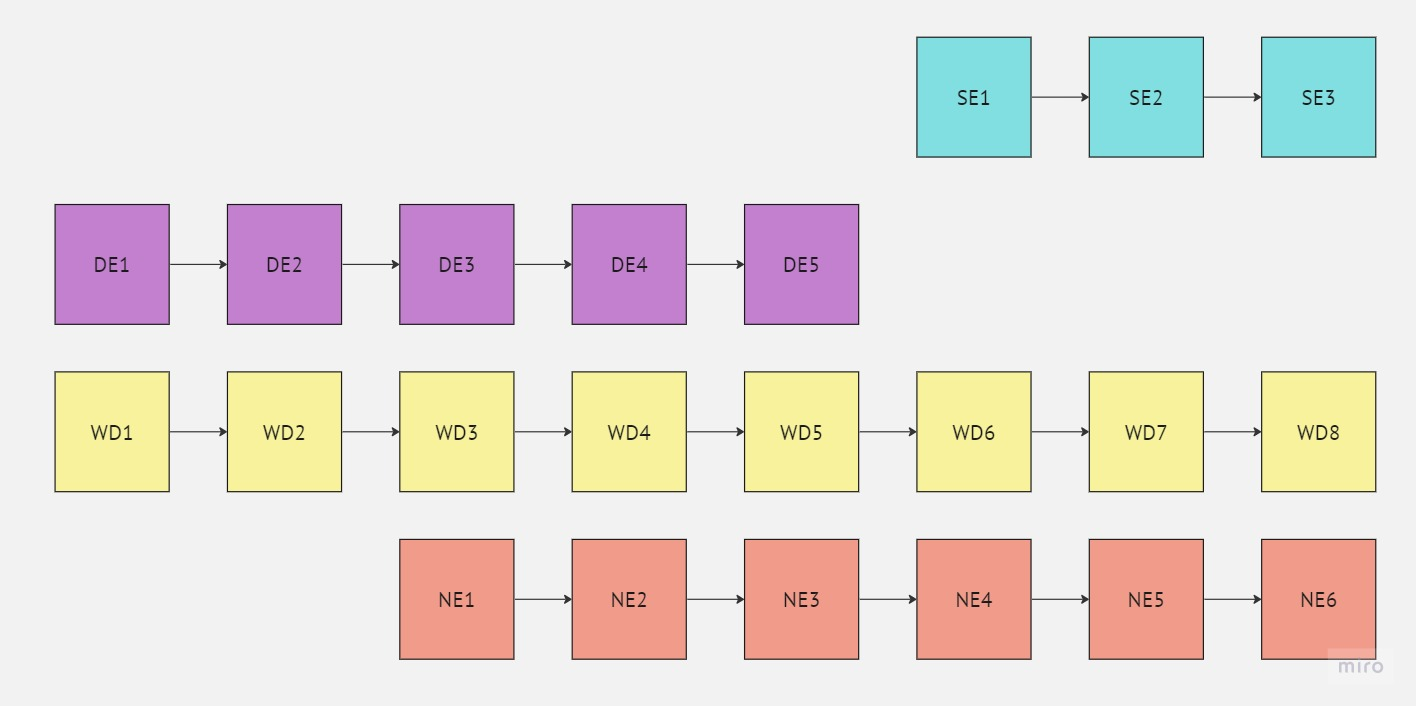
\includegraphics[width=\linewidth]{img/flowchart-development-scholars.jpg}
	\caption{Stappenplan voor de ontwikkeling van het component voor scholieren.}
	\label{img:stappenplan-scholars}
\end{figure}

\begin{center}
	\begin{table}
		\begin{tabular}{ | m{2cm} | m{12cm} | } 
			\hline
			WD1 & Flask-skelet aanmaken \\
			WD2 & Formulier voor GPT-3 API-sleutel invoer maken + sessie \\
			WD3 & Formulier voor gepersonaliseerde opties van website aanmaken + sessie \\
			WD4 & Webpagina's aanmaken in HTML \& CSS \\
			WD5 & Invoerformulier maken voor PDF- en tekstupload \\
			WD6 & JavaScript-functies schrijven voor het weergeven van grammaticale structuren, bijvoeglijke en zelfstandige naamwoorden. \\
			WD7 & JavaScript functies schrijven voor dynamische tekstaanpassing met placeholder-tekst \\
			WD8 & API-calls schrijven voor de functies: look-up, lexicale vereenvoudiging, formaatwijzigingen en ten slotte prompt-gedreven tekstvereenvoudiging \\
			\hline
		\end{tabular}
		\caption{Taken van NLP engineer bij het uitwerken van het scholierencomponent.}
		\label{table:tasks-nlp-engineer-scholars}
	\end{table}
\end{center}

\begin{center}
	\begin{table}[H]
		\begin{tabular}{|m{2cm}|m{12cm}|}
			\hline
			DE1	& Python-notebook om PDFMiner uit te testen bij willekeurige wetenschappelijke artikelen (2000 - nu) \\
			DE2 & Python-notebook opstellen om EasyOCR uit te testen bij willekeurige wetenschappelijke artikelen \\
			DE3 & Jupyter notebook om tekstdata cleaning te realiseren. De restanten van de PDF-extractie moeten weg. \\
			DE4 & Jupyter notebook om look-up methode voor synoniemen te realiseren. \\
			DE5 & Code in back-end implementeren voor PDF-upload via in-memory PDF read. \\
			\hline
		\end{tabular}
		\caption{Taken van data engineer bij het uitwerken van het scholierencomponent.}
		\label{table:tasks-data-engineer-scholars}
	\end{table}
\end{center}